\chapter{Webserver}

\section{Ethernet Shield}\index{Ethernet Shield}

% \lipsum[1-7] % Dummy text

We beginnen dit hoofdstuk met de laatste opdracht van \textit{Programmeren 1}, de “uitsmijter” van de introductie in embedded systems en embedded programming: de Arduino met IO-webserver.

\subsection*{inleiding}
Als onderdeel van de Arduino software worden diverse software-componenten meegeleverd in de vorm van specifieke libraries (documenten -> urduino -> libraries). Controleer dat. Standaard wordt er, bijvoorbeeld, een servo-library, meegeleverd waarmee het werken met servo’s sterk wordt vereenvoudigd. Op vergelijkbare wijze kan voor de ethernet-shield een webserver (component) op poort 80 worden geconfigureerd: \newline

\lstinputlisting[language=Arduino]{code/chapter01/webserver.ino}
$\\$
\begin{exercise}
$\\$ Plaats de Arduino ethernetshield op de Arduino UNO en download het bijbehorende programma (Arduino script, iowebserver.ino) via blackboard en laadt het in je Arduino.
\end{exercise}

\begin{exercise}
$\\$ Sluit je ethernetshield aan op je laptop of (beter nog) op een router, waar uiteraard ook je laptop aan hangt (bedraad of draadloos). \newline
Onderzoek wat het (bedrade) IP-adres van je laptop is en noteer dit. \newline 
Merk op dat je laptop naast de bedrade aansluiting ook nog verbonden kan zijn met het internet via de draadloze verbinding. Dat is handig, want dan kun je ondertussen stackoverflow raadplegen. \newline 
Een directe (doorgaans bedrade) verbinding tussen twee systemen noemt men een ad hoc-netwerk. In beide gevallen, ad hoc of via een router, is het verstandig de netwerkadressen te kiezen in het segment $192.168.1.x$, waarbij $x$ het computernummer is. Het voordeel van dit segment is dat het strikt lokaal is. De informatie van computers in dit segment worden niet doorgegeven over het internet. 
\end{exercise}

\begin{exercise}
$\\$ Bestudeer het webserver-programma en onderzoek of je webserver een IP-adres krijgt en zo ja, welke? \newline
Gebruik de Serial Monitor. Noteer dit adres ook en vergelijk het met dat van je laptop. \newline 
Zitten beide systemen in hetzelfde netwerk(segment)? \newline \newline

De toekenning in de Arduino kan statisch of dynamisch, via DHCP. Welke gebruik je? \newline 
Zorg er hierbij voor dat je in een gecontroleerde netwerkomgeving werkt, met bijvoorbeeld een eigen router waarvan je de instelling kunt aanpassen. \newline
Op het NHL-netwerk hebt je weinig vat, wat aanleiding kan vormen tot problemen (met firewalls etc.). Bij de statische configuratie bepaal je zelf wat het IP-nummer is. Je kunt het (in Windows) aanpassen via het configuratiescherm. \newline
Een nadeel van een statisch IP is dat je, in een netwerk met meerder computer, conflicten kunt krijgen. Beter is het dan ook je Arduino via DHCP een IPnummer te laten toekennen. Dit wordt ondersteund door de serversoftware.
\end{exercise}

Voor de rest van deze opgave gaan we uit van de volgende configuratie: de laptop krijgt adres $192.168.1.2$ en de Arduino(server) $192.168.1.3$. Dat kan bij jou dus, zeker als je DHCP gebruikt, anders zijn. \newline

Probeer, nu je begrijpt hoe eenvoudige netwerkcommunicatie, op het niveau van de IP (-nummers), werkt, de webpagina die is voorgeprogrammeerd in de Arduino-webserver, via je browser zichtbaar te maken door de volgende URL in de voeren:\newline
\url{http://192.168.1.3} \newline
Zie figuur \ref{fig:webserver} voor hoe de site eruit hoort te zien. Mocht dit niet gebeuren en je weet zeker dat alle IP-adressen kloppen, lees dan verder bij de opmerking onderaan deze opdracht.

\begin{figure}[h!]
\centering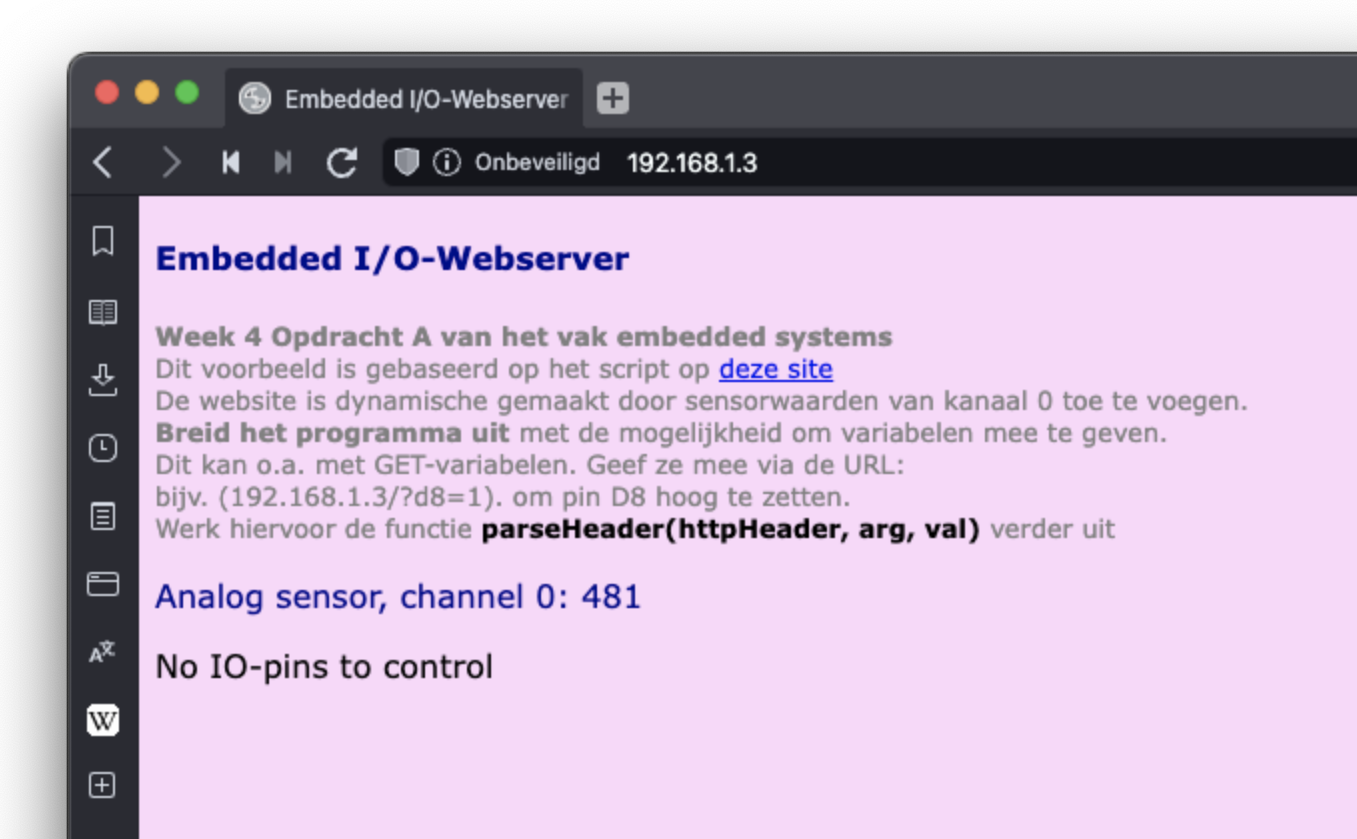
\includegraphics[scale=0.25]{Pictures/chapter01/webserver.png}
\caption{Webserver}
\label{fig:webserver} % Unique label used for referencing the figure in-text
\addcontentsline{toc}{figure}{Figure \ref{fig:webserver}} % Uncomment to add the figure to the table of contents
\end{figure}
